This chapter details the ways the \ac{ahci} driver can be 
run and elaborates on the adjustments needed to be able to 
run the driver on real hardware.

\section{QEMU}

Since version 0.14, QEMU contains an emulation layer for an \acs{ich}-9
\ac{ahci} controller\footnote{The QEMU 0.14 changelog is available at
\url{http://wiki.qemu.org/ChangeLog/0.14}}. To define a disk, the QEMU command
line needs to be extended with:

\begin{lstlisting}[language=bash]
 -device ahci,id=ahci -device ide-drive,drive=disk,bus=ahci.0 \
 -drive id=disk,file=/path/to/disk.img,if=none
\end{lstlisting}

QEMU emulates an \acs{ich}-9 controller sufficiently well that little special
code is required. A first workaround is needed for finding the \ac{ahci}
\acs{pci} \ac{bar}; since the QEMU \ac{ahci} emulation layer does not provide
the legacy IDE compatibility mode, the \ac{ahci} MMIO region is found in
\ac{bar} 0 instead of \ac{bar} 5. Another workaround is necessary when
receiving the response for an {\tt IDENTIFY}, which is a PIO command but is
delivered as a Device to Host Register \ac{fis} by QEMU.

\section{Physical Hardware}

Running Barrelfish on real hardware, one can run into several issues. In order
to be able to test our \ac{ahci} implementation, we had to adjust several
aspects of Barrelfish outside the scope of the \ac{ahci} driver infrastructure.
This chapter details any additional modifications.

\subsection{PCI Base Address Registers}

Barrelfish's system knowledge base is not able to handle addresses above 32 bit
correctly. Fixing this issue would require extensive modifications in the
\acs{skb} which are out of the scope of this lab project. As a consequence,
\emph{ahcid} will receive zero \acp{bar} on hardware where the \ac{ahci} memory
regions are mapped in memory above 4GB and thus be unable to access the memory
mapped I/O region to control the \ac{hba}. For the same reason, the code produced by
this lab project has not been tested for 64bit addresses in memory mapped I/O
regions.  Still, once the issues in the \acs{hba} have been fixed, the driver should
properly recognise and handle the devices in question.

\subsection{PCI Bridge Programming}

Because of a bug in \acs{pci} bridge programming, Barrelfish sometimes does not
program \acs{pci} \acp{bar} correctly if \acs{pci} bridges are present. For
this lab project, we introduce a workaround that will retrieve the original
\acp{bar} in case no reprogrammed \acp{bar} can be found in the \acs{skb}.

This is achieved in the \lstinline+device_init+ function of \lstinline+pci.c+,
by querying the \acs{skb} for the original \lstinline+bar(...)+ facts of the
device if no reprogrammed ones can be found:

\begin{lstlisting}
error_code = skb_execute_query(
  "findall(baraddr(BAR,Base,0,Size),bar(addr(%u,%u,%u)"
  ",BAR,Base,Size,_,_,_), BARList),"
  "sort(1, =<, BARList, L),"
  "length(L,Len),writeln(L)",
  *bus, *dev, *fun);
\end{lstlisting}

The result of this prolog expression has exactly the same form as
\lstinline+pci_get_+\linebreak \lstinline+implemented_BAR_addresses+ therefore
the surrounding code is exactly the same as in the usual case.

\subsection{BIOS Memory Maps}

On x86 architectures, the BIOS memory map can be retrieved to determine the
layout of memory. Some BIOSs report a memory map that is not sorted by
increasing base address or even might return overlapping and conflicting memory
regions.  This lab project contains modifications to the code that creates
capabilities to physical memory in \verb+startup_arch.c+ such that the memory
map is preprocessed to eliminate conflicts and ensure ascending addresses.

As the preprocessed memory map might be larger due to the case where one memory
region completely contains another and thus is split into three new regions, we
first need to copy the map into a larger buffer. The memory map is then sorted
with a simple bubblesort.  To remove conflicts, overlapping regions are given
to the region with the higher type or merged if they are both of the same type.
At the end, regions are page-aligned as Barrelfish can only map whole pages.

\autoref{fig:mmap} shows the memory maps seen on a DELL Optiplex 755
workstation. Several regions are not aligned to the pagesize and the region at
\lstinline+0xfec00000+ does not appear in ascending order. After preprocessing,
memory addresses appear in ascending order and are page-aligned. Note that
higher types take precedence, therefore page alignment does not necessarily
round down.

\begin{figure}[ht]
\centering
\includegraphics[width=.7\textwidth]{mmap.pdf}
\caption{Memory map transformation}
\label{fig:mmap}
\end{figure}
